\documentclass[letterpaper]{article}
\usepackage{uai2019}
\usepackage[margin=1in]{geometry}

% Set the typeface to Times Roman
\usepackage{times}
\usepackage[utf8]{inputenc}
\usepackage{mathtools}
\usepackage{amsfonts}
\usepackage{booktabs}
\usepackage[colorlinks=true,citecolor=blue,urlcolor=blue]{hyperref}

\newcommand{\mean}[1]{\left\langle #1 \right\rangle}
\newcommand{\avg}[1]{\langle#1\rangle}
\newcommand{\et}{\;\mathrm{and}\;}
\newcommand{\Real}{\mathbb{R}}
\newcommand{\STAB}{\mathrm{STAB}}
\renewcommand{\TH}{\mathrm{TH}}
\newcommand{\chull}{\mathrm{Conv}}

\begin{document}
\title{Supplemental Materials}
\maketitle
%\section*{Detailed description of the method}
\section*{Edge colored multigraph technique for approximating the quantum
bound}
\begin{figure}[t]
    \centering
    \includegraphics[width=.7\columnwidth]{images/instrumental_multigraph.pdf}
    \caption{Edge colored exclusivity graph representation of the Bonet
        inequality. Exclusivity constraints for the party $A$ and $B$ are
    represented by red lines and blue lines respectively.}
    \label{fig:instrumental_multigraph}
\end{figure}
Applying the technique described above to this scenario yields a quantum
bound of $2.2071$, reproducing the known value for the quantum bound of the Bonet inequality given by $(3+\sqrt{2})/2$.

The Lovasz theta of a graph, despite being efficiently computable, only gives an upper bound to the maximal quantum bound, since it ignores the additional constraints arising from the presence of different parties. To obtain a better approximation for the quantum bound we follow the technique presented
in \cite{rabelo2014}. This method consists in introducing an edge coloring in the exclusivity graph. It encodes the information of which of the parties is being employed to arrive at the exclusivity constraints under consideration. This effectively corresponds to constructing an exclusivity graph $G_i$ for each
party, the resulting object is called a \emph{multigraph}. Having defined a multigraph $G = {G_1, \ldots, G_n}$ for a given scenario the
quantum bound is defined by the quantity:
\begin{equation}
    \vartheta(G) = \max_{v} \sum_{i \in V} |v \cdot a^1_i \otimes \dots \otimes a^n_i|^2
    \label{eq:multigraph_lovazs}
\end{equation}
where $\{a^j_i\}$ is an orthonormal labelling for $G_j$ and $V$ is the set of vertices of $G$. This quantity, which can be seen as a generalization of the Lov\'asz theta, is in general not efficiently computable, but can be arbitrarily approximated by a hierarchy of semi-definite programs as described in \cite{rabelo2014}.
In the case of the pentagon in the instrumental scenario we have two colors, and thus two graph $G_A$ and $G_B$, corresponding to party $A$ and $B$ respectively, as shown in Fig.~\ref{fig:instrumental_multigraph}.

\section*{There are no quantum violation for instrumental scenarios with $l=2$
settings.}
Here we prove that no quantum violation is possible for instrumental scenario
with $l=2$ possible settings for the instrumental variable $X$.
This reduces to proving that there are no odd $n$-cycles nor $n$-anticycles as induced
subgraphs in the corresponding exclusivity graph, with $n\ge5$.
To see this we can notice that any such graph is composed by two cliques (see
for example Fig.~\ref{fig:2mn_nocycle_proof}), corresponding to the events with $x=0$ and
$x=1$.
\begin{figure}[t]
    \centering
    \includegraphics[width=.7\columnwidth]{images/nocycles_proof.pdf}
    \caption{Exclusivity graph for the instrumental scenario $233$, showing the
        impossibility of having cycles with more than $5$ vertices. To simplify the figure cliques are
    represented by bold lines between vertices.}
    \label{fig:2mn_nocycle_proof}
\end{figure}
Any $n$-cycle with at least $5$ vertices must then have at least $3$ mutually
connected vertices belonging to the same $x$, so they can never form a
cycle-graph.
Similarly we can show that there cannot be any induced odd anticycle with $5$ or more
vertices.

\section*{There are no cycles $C_n$ with $n \ge 7$ in the $l22$ instrumental scenario.}
%\label{sec:c5only_proof}
In the following we prove that there cannot be a odd anticycle with more than
$5$ vertices in the exclusivity graph associated to an instrumental scenario of
the type $l22$.

\begin{figure}[h]
    \centering
    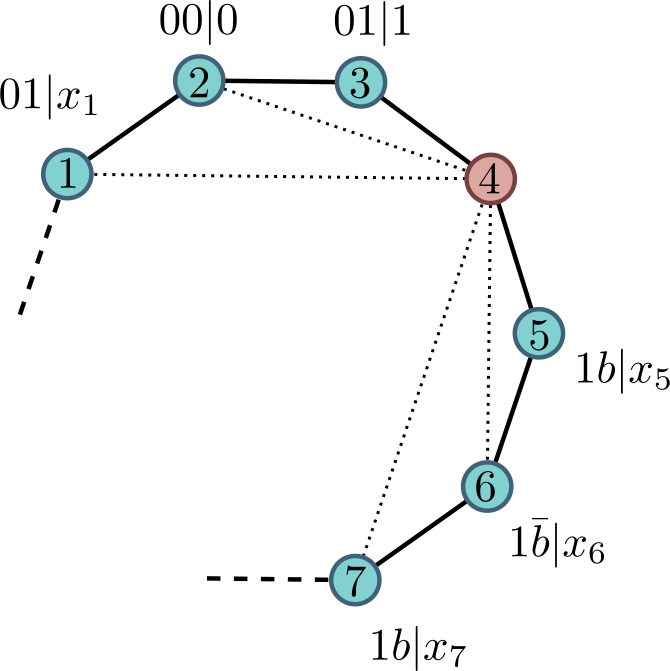
\includegraphics[width=.6\columnwidth]{images/cycle_proof.pdf}
    \caption{Proof of the impossibility of having cycles with $7$ nodes or more
    in the $d22$ scenario.}
    \label{fig:cycle_graph_proof}
\end{figure}

From the exclusivity conditions \eqref{eq:non_exclusivity_condition},
given two events $ab|x$ and $a'b'|x'$, they are connected by edge if one of these two conditions is true:
\begin{enumerate}
    \item $x=x'$.\label{en:rule1}
    \item $a=a'$ and $b \neq b'$.\label{en:rule2}
\end{enumerate}
Suppose we have a cycle $C_n$ with $n \ge 7$, as in fig.~\ref{fig:cycle_graph_proof},
and consider that node $2$ in this graph corresponds to an event which we can arbitrarily identify as $00|0$.
Among its neighbors $1$ and $3$, one will necessarily need to satisfy rule
\ref{en:rule2} (they cannot both satisfy rule \ref{en:rule1} or the three nodes
would be a clique.
%TODO: Explain what is a clique.
So without loss of generality we can assign the event $01|1$ to $3$.
Since nodes $5,6,7$ must not satisfy rule \ref{en:rule2} with both $2$ and $3$, then they must have $a = 1$.
Moreover $7$ and $5$ must have the same $b$, different from $6$. In the same way $1$ must not satisfy rule \ref{en:rule2} with $6,5$ and $3$, so it
needs to have $a=0$ and $b=1$. At this point, since we only have values
$\{0,1\}$ for $a$, we cannot avoid node $4$ to be linked to one of the nodes
$1,2,6,7$. Thus, the corresponding graph cannot be a cycle.
\end{document}
